\clearpage
\section*{\currfilename}

\begin{tikzpicture}
  \node (block3) [squareblock, label=below:{\shortstack[c]{\bf Nonlinear Equations\\ \bf of Motion}}, minimum width=6cm, inner sep=0mm] {\centering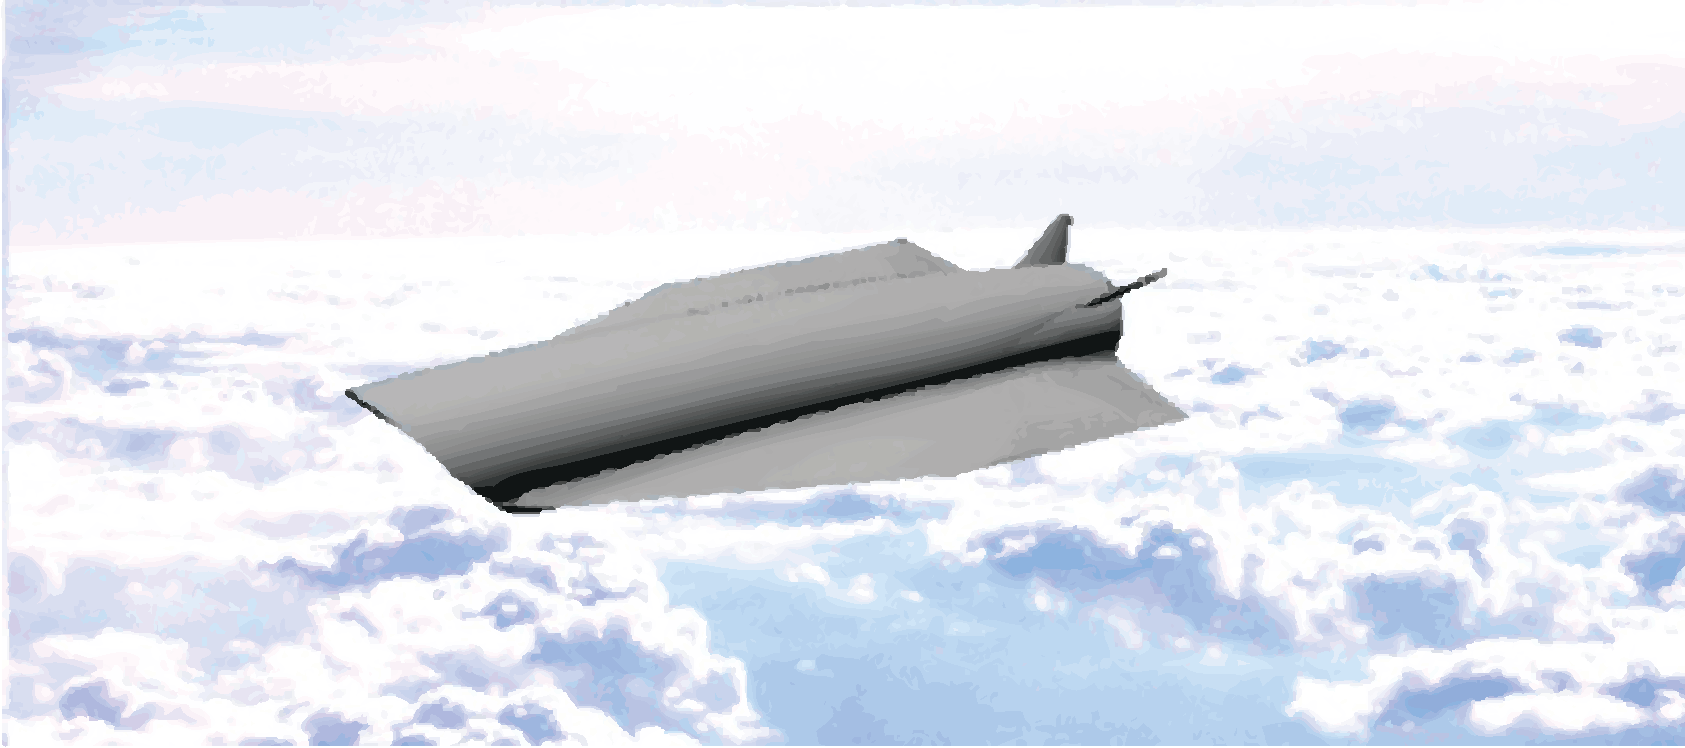
\includegraphics[width=6cm]{../fig/ghvclouds.pdf}};
  \path (naveq.145)+(-\blockdist,0) node (block1) [squareblock, minimum width=2.5cm] {Baseline};
  \path (naveq.-145)+(-\blockdist,0) node (block2) [squareblock, minimum width=2.5cm] {\shortstack{Adaptive \\ Augmentation}};
  \node[squareblock, below of=block2, node distance=1.5cm, minimum height=1cm, minimum width=2cm] (blockT){\fontsize{14pt}{14pt}\selectfont$\theta(t)$};
  \node[squareblock, minimum height=1cm, minimum width=2cm, right of=block3, node distance=5.0cm] (block4) {\shortstack[c]{Error \\ Generator}};
  \node[output, right of=block4,node distance=2.0cm] (output1) {};
  \node[input, below of=blockT, node distance=1.5cm] (input2) {};
  \path [draw, ->] (block1) -- (block3.west |- block1) ;
  \path [draw, ->] (block2) -- (block3.west |- block2);
  \draw[->](input2) -- node[left,pos=0.5]{$e$, $x$, $\Gamma$}(blockT);
  \draw[->](blockT) -- (block2);
  \draw[->](block3) -- (block4);
  \draw[->](block4) --  node[above,pos=0.8]{$e$}(output1);
\end{tikzpicture}

% \node (output1) [input, right of=sum1, node distance=1.5cm] {};
% \path [draw, ->] (block1) -- (block3.west |- block1) ;
% \path [draw, ->] (block2) -- (block3.west |- block2);
% \path [draw, ->] (block3) -- node[pos=0.7]{$-$} (sum1);
% \path [draw, ->] (input1) -- node[pos=0.2]{target} node[pos=0.7]{$+$} (sum1);
% \path [draw, ->] (sum1) -- node[pos=0.7]{error} (output1);
% \draw[->](block3) -- node[pos=0.7, anchor=north]{$-$} (sum1);
